% SPDX-License-Identifier: AGPL-3.0-or-later
% Commercial license available
% © Concepts 1996-2026 Miroslav Sotek. All rights reserved.
% © Code 2020-2026 Miroslav Sotek. All rights reserved.
% ORCID: 0009-0009-3560-0851
% Contact: www.anulum.li | protoscience@anulum.li
% scpn-quantum-control --- Phase 3 entanglement/tomography short paper

\documentclass[preprint,aps,physrev,superscriptaddress,floatfix,longbibliography]{revtex4-2}

\usepackage{amsmath,amssymb}
\usepackage{booktabs}
\usepackage{graphicx}
\usepackage{hyperref}
\usepackage{xcolor}
\usepackage{xurl}
\usepackage{siunitx}

\hypersetup{
    colorlinks=true,
    linkcolor=blue!60!black,
    citecolor=blue!60!black,
    urlcolor=blue!60!black,
}

\begin{document}
\emergencystretch=3em

\title{Reduced-Pauli entanglement checks for DLA-sector leakage mechanisms on IBM Heron hardware}

\author{Miroslav \v{S}otek}
\email{protoscience@anulum.li}
\affiliation{ANULUM, Marbach SG, Switzerland}
\affiliation{ORCID: 0009-0009-3560-0851}

\date{\today}

\begin{abstract}
Parity-sector leakage asymmetry in small Kuramoto--XY circuits is a useful
hardware observable only if the mechanism can be separated from layout,
prepared-state, and readout artefacts. We report a cost-bounded reduced-Pauli
entanglement/tomography check for promoted Phase~3 DLA-parity and
Fisher-information-modified Kuramoto--XY circuit families. The approved
\texttt{ibm\_marrakesh} execution used physical qubits $[1,2,3,4]$, 162 main
circuits, four readout calibration circuits, 2048 shots per main circuit, and
8192 shots per readout circuit. The primary submitted IBM jobs were
\texttt{d86g7h1789is738vkreg} and \texttt{d86ggpis46sc73f6v170}. A
preregistered reducer produced 54 observable rows. The mean absolute
measured-minus-exact deviation is 0.1299 and the maximum absolute deviation is
0.5561. The largest deviations are concentrated in transverse two-qubit
correlators, especially DLA odd-sector \texttt{XX}/\texttt{YY} edge channels,
while the FIM lambda-4 circuit deviates more strongly than
the FIM lambda-0 reference. A tensor-product readout-mitigation
replay leaves the primary mean absolute deviation essentially unchanged
(0.1293), and a same-day \texttt{ibm\_fez} replication gives mean absolute
deviation 0.1528, readout-mitigated to 0.1513. A pinned-layout
\texttt{ibm\_fez} repeat with full 16-state readout calibration gives raw mean
absolute deviation 0.1494; correlated readout inversion amplifies rather than
erases the strongest channels, with the largest amplification still
concentrated in transverse edge observables. A preregistered five-channel ZNE
stress test on the same \texttt{ibm\_fez} qubits gives linear-ZNE mean
absolute deviation 0.4412 versus 0.4196 at scale~1, so noise scaling does not
erase the dominant DLA-channel discrepancy. The FIM control channel partially
improves under ZNE, suggesting that the discrepancy is structured rather than
simple monotone gate noise. A third-backend \texttt{ibm\_kingston} ZNE
replication on qubits $[141,142,143,144]$ gives the same qualitative pattern:
the four DLA transverse channels move farther from exact under linear ZNE,
while the FIM control improves. A same-layout Kingston statistical repeat
preserves this DLA-worsens/FIM-improves separation. Larger $n=6,8$
reduced-Pauli/ZNE lanes on Fez and Marrakesh then address the ``all hardware is
$n=4$'' limitation with 36 reduced-Pauli channels per lane. A Kingston
larger-width replication adds the third backend, and a Marrakesh $n=8$ repeat
checks the largest readout-sensitivity effect. The readout-mitigated
linear-ZNE mean absolute deviations range from 0.0980 to 0.1577 on Fez, from
0.0604 to 0.0688 on Marrakesh after a large readout-sensitivity correction,
and from 0.1504 to 1.6735 on Kingston, where the $n=6$ full-readout assignment
matrix is singular and therefore reported with a pseudo-inverse sensitivity
boundary. The result is a
mechanism-boundary measurement:
it shows structured reduced-Pauli distortions accompanying the small-system
DLA/FIM hardware programme, but does not claim scalable tomography, quantum
advantage, full-state reconstruction, or backend-general entanglement
dynamics.
\end{abstract}

\maketitle

\section{Introduction}

Kuramoto synchronisation and XY spin Hamiltonians provide a compact route from
phase-oscillator structure to gate-model quantum
dynamics~\cite{Kuramoto1975,Acebron2005}. The dynamical-Lie-algebra language
used here follows the standard Lie-algebraic controllability framework for
finite-dimensional quantum systems~\cite{DAlessandro2007}.
In the present programme, the relevant small-system hardware question is not
whether a broad advantage has been demonstrated. It is narrower: when
sector-resolved leakage and retention observables deviate from exact
Kuramoto--XY references on IBM hardware, do reduced-Pauli correlators show an
accompanying structure that can constrain the mechanism?

Previous DLA-parity and FIM runs established bounded hardware observations,
including backend, layout, state-preparation, and readout
sensitivity~\cite{SotekDLA2026,SotekFIM2026}. A scalar
leakage metric alone cannot distinguish coherent correlator deformation from
population readout effects or generic depth-dependent decoherence on noisy
intermediate-scale quantum hardware~\cite{Preskill2018}. This paper therefore
measures a small set of preregistered reduced-Pauli observables for the same
class of promoted circuits. Full tomography~\cite{NielsenChuang2010} is
unnecessary for this question, and the protocol is closer in spirit to
targeted local-observable estimation than to full state reconstruction; related
measurement-efficient ideas include classical shadows and local observable
prediction~\cite{HuangKuengPreskill2020}. The aim here is narrower still: to
compare selected two-qubit correlators against exact classical references
under one backend, layout, shot budget, and calibration window.
The contribution is a channel-localised falsifier: the dominant DLA transverse
deviations survive readout replay, backend replication, and ZNE stress tests,
so future mechanism claims must account for correlator-level structure rather
than only scalar leakage summaries.

\section{Protocol}

The source circuits are listed in Table~\ref{tab:sources}. Four DLA-parity
circuits compare even and odd initial states at shallow and signal depths. Two
FIM-pair circuits compare $\lambda_{\mathrm{fim}}=0$ and
$\lambda_{\mathrm{fim}}=4$ at fixed initial state and depth.

\begin{table}[tb]
\centering
\begin{tabular}{lllc}
\toprule
Label & Family & Initial state & Depth \\
\midrule
\texttt{dla\_even\_shallow} & DLA parity & \texttt{0011} & 6 \\
\texttt{dla\_odd\_shallow} & DLA parity & \texttt{0001} & 6 \\
\texttt{dla\_even\_signal} & DLA parity & \texttt{0011} & 10 \\
\texttt{dla\_odd\_signal} & DLA parity & \texttt{0001} & 10 \\
\texttt{fim\_lambda0\_reference} & FIM pair & \texttt{0011} & 4 \\
\texttt{fim\_lambda4\_feedback} & FIM pair & \texttt{0011} & 4 \\
\bottomrule
\end{tabular}
\caption{Promoted source circuits for the reduced-Pauli check.}
\label{tab:sources}
\end{table}

For each source circuit we measure nine reduced-Pauli basis settings,
\begin{equation}
\{\texttt{IIXX},\texttt{IIYY},\texttt{IIZZ},\texttt{IXXI},\texttt{IYYI},
\texttt{IZZI},\texttt{XXII},\texttt{YYII},\texttt{ZZII}\}.
\end{equation}
Each source/basis pair is repeated three times at 2048 shots, giving 162 main
circuits. Four computational-basis readout states, \texttt{0000},
\texttt{0001}, \texttt{0011}, and \texttt{1111}, are measured at 8192 shots.
The complete hardware block therefore contains 166 circuits. The selected
physical qubits are $[1,2,3,4]$ on \texttt{ibm\_marrakesh}; the maximum
transpiled depth in the live preflight is 388, and the maximum
measurement-basis depth expansion is 1.0718. A second-backend replication on
\texttt{ibm\_fez} used physical qubits $[21,22,23,24]$, the same circuit and
shot budget, and jobs \texttt{d86h4jlg7okc73el3ra0} and
\texttt{d86h5d9789is738vlt7g}. A pinned-layout repeat on the same
\texttt{ibm\_fez} qubits added all 16 computational-basis readout calibration
states and used jobs \texttt{d86hdk8p0eas73dkv9eg} and
\texttt{d86hedp789is738vm7mg}. Circuit construction, transpilation, and
hardware execution used Qiskit and the IBM Quantum
platform~\cite{Qiskit2024,IBMQuantum}.

After the \texttt{ibm\_fez} ZNE stress test, we executed a third-backend ZNE
replication on \texttt{ibm\_kingston}. The selected physical qubits were
$[141,142,143,144]$. The run used the same preregistered five channels, the
same global unitary-folding scale factors $1,3,5$, the same three repetitions
per channel and scale, 2048 main shots, and full 16-state readout calibration
at 8192 shots. The completed jobs were \texttt{d86i8fas46sc73f70vg0} and
\texttt{d86ijr9789is738vnh30}. A same-layout statistical repeat used jobs
\texttt{d86pul0p0eas73dla3dg} and \texttt{d86pul8p0eas73dla3eg}.

\section{Analysis}

For each measured basis-rotated circuit, the reducer estimates the Pauli
expectation
\begin{equation}
  \langle P \rangle =
  \frac{1}{N}\sum_b n_b
  \prod_{i\in \mathrm{supp}(P)} (-1)^{b_i},
\end{equation}
where $P$ is the reduced-Pauli label, $n_b$ is the observed count for bitstring
$b$, and $N$ is the total shot count. Repetitions are grouped by source label
and basis setting, then compared with exact reference expectations from the
committed reference table
\path{data/phase3_entanglement_tomography/entanglement_observable_rows_2026-05-07.csv}.

The primary output rows are committed in
\path{data/phase3_entanglement_tomography/entanglement_tomography_rows_2026-05-20.csv}.
The rows have SHA256 digest
\path{b280db120f9f13dfb8dd6b8d4e2e6a86a86feff714e2514be01bd5b3ed95bd83}.

Readout mitigation is applied as a conservative replay, not as a stronger
hardware claim. The four calibration circuits are marginalised into independent
single-qubit assignment matrices in IBM count-key order, and the tensor-product
assignment matrix is inverted before recomputing each reduced-Pauli
expectation, following the standard response-matrix/post-processing
measurement-error mitigation logic~\cite{Maciejewski2020}. This is not a full
16-state correlated readout calibration and is not ZNE or PEC. When all 16
calibration states are present in the pinned
\texttt{ibm\_fez} repeat, the reducer instead inverts the full correlated
16-by-16 assignment matrix. This still corrects only readout assignment; it
does not correct basis rotations, coherent gate errors, drift, or depth
effects.

\section{Results}

The approved IBM execution completed on \texttt{ibm\_marrakesh}. The submitted
jobs were \texttt{d86g7h1789is738vkreg} and
\texttt{d86ggpis46sc73f6v170}. The analysis produced 54 observable rows with
mean absolute deviation 0.1299 and maximum absolute deviation 0.5561 relative
to exact references.

Table~\ref{tab:label-summary} gives the label-level aggregates. DLA circuits
have larger mean absolute deviation than the FIM pair overall. Within the DLA
family, the odd shallow and odd signal circuits produce the largest aggregate
departures. Within the FIM pair, $\lambda_{\mathrm{fim}}=4$ has more than twice
the mean absolute deviation of $\lambda_{\mathrm{fim}}=0$.

\begin{table}[tb]
\centering
\small
\begin{tabular}{lrrr}
\toprule
Circuit label & Mean signed & Mean absolute & Max absolute \\
\midrule
\texttt{dla\_even\_shallow} & -0.120474 & 0.148396 & 0.314180 \\
\texttt{dla\_even\_signal} & 0.061095 & 0.063458 & 0.160443 \\
\texttt{dla\_odd\_shallow} & 0.098416 & 0.219708 & 0.515473 \\
\texttt{dla\_odd\_signal} & 0.153497 & 0.176026 & 0.556091 \\
\texttt{fim\_lambda0\_reference} & 0.030496 & 0.052205 & 0.088148 \\
\texttt{fim\_lambda4\_feedback} & 0.096107 & 0.119566 & 0.274155 \\
\bottomrule
\end{tabular}
\caption{Label-level measured-minus-exact deviation aggregates. Each row
summarises nine reduced-Pauli observables.}
\label{tab:label-summary}
\end{table}

Figure~\ref{fig:heatmap} shows the signed measured-minus-exact deviations by
source label and basis setting. The strongest pattern is not a uniform decay of
all correlators. Instead, deviations concentrate in transverse two-qubit
channels. The odd-sector DLA signal circuit has large positive shifts in
\texttt{XXII} and \texttt{YYII}; the odd shallow circuit has analogous positive
shifts in \texttt{IIXX} and \texttt{IIYY}. The even shallow circuit moves in
the opposite direction on corresponding transverse channels.

\begin{figure}[tb]
\centering
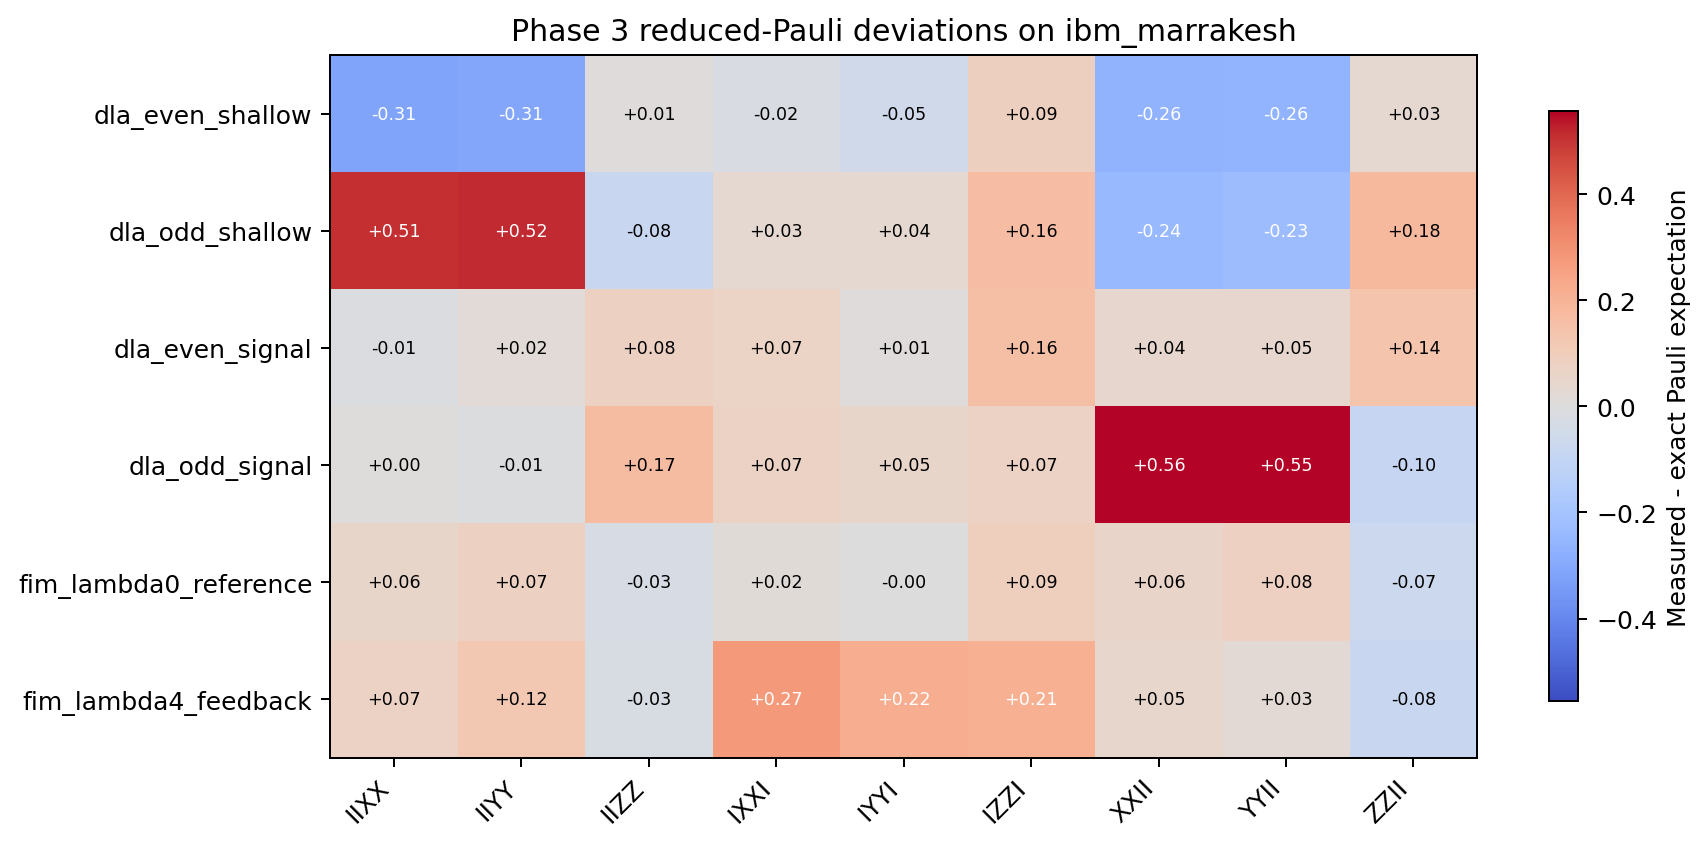
\includegraphics[width=0.98\linewidth]{figures/phase3/phase3_entanglement_deviation_heatmap_2026-05-20.png}
\caption{Measured-minus-exact reduced-Pauli deviations for the completed
\texttt{ibm\_marrakesh} run. The strongest deviations concentrate in
transverse edge correlators rather than in all observables uniformly.}
\label{fig:heatmap}
\end{figure}

The largest individual deviations are shown in Table~\ref{tab:top}. The top
four are DLA odd-sector transverse correlators. The strongest FIM-channel
departure is the \texttt{IXXI} observable for the
$\lambda_{\mathrm{fim}}=4$ circuit.

\begin{table}[tb]
\centering
\small
\begin{tabular}{llrrr}
\toprule
Circuit label & Basis & Measured & Exact & Deviation \\
\midrule
\texttt{dla\_odd\_signal} & \texttt{XXII} & 0.431641 & -0.124450 & 0.556091 \\
\texttt{dla\_odd\_signal} & \texttt{YYII} & 0.429688 & -0.124450 & 0.554138 \\
\texttt{dla\_odd\_shallow} & \texttt{IIYY} & 0.488932 & -0.026541 & 0.515473 \\
\texttt{dla\_odd\_shallow} & \texttt{IIXX} & 0.478841 & -0.026541 & 0.505382 \\
\texttt{dla\_even\_shallow} & \texttt{IIXX} & -0.456055 & -0.141874 & -0.314180 \\
\texttt{dla\_even\_shallow} & \texttt{IIYY} & -0.447591 & -0.141874 & -0.305717 \\
\texttt{fim\_lambda4\_feedback} & \texttt{IXXI} & 0.175781 & -0.098373 & 0.274155 \\
\bottomrule
\end{tabular}
\caption{Largest measured-minus-exact deviations in the reduced-Pauli rows.}
\label{tab:top}
\end{table}

\subsection{Readout mitigation and same-day replication}

Table~\ref{tab:backend-comparison} summarises the primary
\texttt{ibm\_marrakesh} run, the same-day \texttt{ibm\_fez} replication, and
the pinned-layout \texttt{ibm\_fez} repeat with full readout calibration.
The tensor-product readout inversion does not collapse the deviations toward
zero on either backend. On \texttt{ibm\_marrakesh}, the mean absolute deviation
changes from 0.1299 to 0.1293; on \texttt{ibm\_fez}, it changes from 0.1528 to
0.1513. The pinned-layout repeat gives a similar raw mean absolute deviation,
0.1494, while full correlated readout inversion increases the aggregate
mitigated deviation to 0.1953 and the largest mitigated deviation to 0.9913.
This does not prove backend-general dynamics, but it does rule out the simplest
interpretation that the primary observation is only a single-backend
population-readout artefact. The full correlated inversion result is treated as
a sensitivity bound, because matrix inversion can amplify calibration and shot
noise in individual channels.

The amplification is not uniform across the reduced-Pauli table. In the
pinned full-readout replay, transverse edge channels have mean absolute
amplification 0.1110 and maximum amplification 0.5178, while transverse-middle
channels have mean absolute amplification 0.0026. The two largest amplified
rows are \texttt{dla\_odd\_shallow}/\texttt{IIYY} and
\texttt{dla\_odd\_shallow}/\texttt{IIXX}, both already in the dominant
DLA transverse-edge family. The \texttt{ZZ} edge class also shows
sensitivity, with mean absolute amplification 0.0946 and maximum
amplification 0.2855. Thus the correlated-inversion replay should not be read
as a clean mitigation result, but it also does not look like a featureless
uniform noise blow-up. The supplementary amplification rows are generated in
\path{data/phase3_entanglement_tomography/entanglement_tomography_full_readout_amplification_top_2026-05-20.csv}
and
\path{data/phase3_entanglement_tomography/entanglement_tomography_full_readout_amplification_classes_2026-05-20.csv}.

\begin{table}[tb]
\centering
\small
\begin{tabular}{lrrrr}
\toprule
Backend & Mean abs. & Max abs. & Mitigated mean abs. & Mitigated max abs. \\
\midrule
\texttt{ibm\_marrakesh} & 0.129893 & 0.556091 & 0.129304 & 0.564834 \\
\texttt{ibm\_fez} auto layout & 0.152821 & 0.479015 & 0.151317 & 0.486875 \\
\texttt{ibm\_fez} pinned full readout & 0.149445 & 0.473481 & 0.195282 & 0.991278 \\
\bottomrule
\end{tabular}
\caption{Cross-backend reduced-Pauli deviation summary. Mitigation is
independent single-qubit readout inversion for the first two rows and full
correlated readout inversion for the pinned full-readout row.}
\label{tab:backend-comparison}
\end{table}

\subsection{ZNE stress test}

After the full-readout replication, we executed the preregistered ZNE subset
proposed by the mechanism-boundary analysis. The run used \texttt{ibm\_fez}
qubits $[21,22,23,24]$, global unitary-folding scale factors $1,3,5$, three
repetitions per channel and scale, and the full 16-state readout calibration.
This follows the short-depth error-mitigation and digital ZNE framework
~\cite{Temme2017,LiBenjamin2017,Endo2021,GiurgicaTiron2020}.
The submitted jobs were \texttt{d86hs6qs46sc73f70h90} and
\texttt{d86hsltg7okc73el4lg0}. The resulting artefact contains 45 main
circuits and 16 readout-calibration circuits. The ZNE reducer groups rows by
channel and noise scale, computes raw and full-correlated-readout-mitigated
expectations, and performs linear and quadratic extrapolations to zero noise.

Table~\ref{tab:zne} gives the channel-level summary. The aggregate result is a
negative mitigation outcome for the DLA channels: the scale-1 mean absolute
deviation across the five selected channels is 0.4196, while linear ZNE gives
0.4412 and full-readout-mitigated linear ZNE gives 0.4468. The four DLA
transverse channels all move farther from the exact reference under linear
ZNE. The FIM control behaves differently: \texttt{fim\_lambda4\_feedback}/
\texttt{IZZI} improves from scale-1 deviation 0.4508 to linear-ZNE deviation
0.4170, and the quadratic fit gives 0.2294. Because quadratic extrapolation
with three scales can overfit the three points, it is reported as a sensitivity
check rather than a stronger correction claim.

The third-backend \texttt{ibm\_kingston} replication gives the same qualitative
channel separation, as shown in Table~\ref{tab:zne-kingston}. The scale-1 mean
absolute deviation is 0.4534, linear ZNE gives 0.4729, and
full-readout-mitigated linear ZNE gives 0.4806. All four DLA transverse
channels again move farther from exact under linear ZNE. The FIM control moves
in the opposite direction, improving from scale-1 deviation 0.2490 to
linear-ZNE deviation 0.1673 and quadratic-ZNE deviation 0.0490. This is not a
backend-general dynamics claim, but it is a third-backend qualitative
replication of the Fez stress-test pattern under the same five-channel
protocol. The same-layout Kingston repeat preserves the pattern: scale-1 mean
absolute deviation is 0.4656, linear ZNE gives 0.4816, and
full-readout-mitigated linear ZNE gives 0.4893. In the repeat, all four DLA
transverse channels again move farther from exact under linear ZNE, while the
FIM control improves from scale-1 deviation 0.2564 to linear-ZNE deviation
0.1941.

\begin{table}[tb]
\centering
\small
\begin{tabular}{llrrr}
\toprule
Circuit label & Basis & Scale-1 abs. & Linear ZNE abs. & Mitigated linear abs. \\
\midrule
\texttt{dla\_odd\_shallow} & \texttt{IIXX} & 0.490083 & 0.524344 & 0.535976 \\
\texttt{dla\_odd\_shallow} & \texttt{IIYY} & 0.457531 & 0.493067 & 0.503956 \\
\texttt{dla\_odd\_signal} & \texttt{XXII} & 0.340596 & 0.378709 & 0.386027 \\
\texttt{dla\_odd\_signal} & \texttt{YYII} & 0.359151 & 0.393086 & 0.400958 \\
\texttt{fim\_lambda4\_feedback} & \texttt{IZZI} & 0.450778 & 0.417032 & 0.407170 \\
\bottomrule
\end{tabular}
\caption{Preregistered ZNE stress-test summary on \texttt{ibm\_fez}. The
table reports absolute deviation from exact reference at scale~1, after
linear extrapolation from scale factors $1,3,5$, and after full-correlated
readout inversion followed by linear extrapolation.}
\label{tab:zne}
\end{table}

\begin{table}[tb]
\centering
\small
\begin{tabular}{llrrr}
\toprule
Circuit label & Basis & Scale-1 abs. & Linear ZNE abs. & Mitigated linear abs. \\
\midrule
\texttt{dla\_odd\_shallow} & \texttt{IIXX} & 0.501476 & 0.525673 & 0.541006 \\
\texttt{dla\_odd\_shallow} & \texttt{IIYY} & 0.508963 & 0.546913 & 0.563012 \\
\texttt{dla\_odd\_signal} & \texttt{XXII} & 0.504333 & 0.571200 & 0.583571 \\
\texttt{dla\_odd\_signal} & \texttt{YYII} & 0.503031 & 0.553459 & 0.565459 \\
\texttt{fim\_lambda4\_feedback} & \texttt{IZZI} & 0.248955 & 0.167331 & 0.149998 \\
\bottomrule
\end{tabular}
\caption{Third-backend ZNE replication on \texttt{ibm\_kingston}. The
five-channel protocol is identical to Table~\ref{tab:zne}; all four DLA
transverse channels worsen under linear ZNE, while the FIM control improves.}
\label{tab:zne-kingston}
\end{table}

\subsection{Larger-width reduced-Pauli stress lanes}

To avoid leaving the hardware package entirely at $n=4$, we executed a bounded
larger-width extension on \texttt{ibm\_fez} and \texttt{ibm\_marrakesh} at
$n=6$ and $n=8$. The larger lanes retain the reduced-Pauli philosophy rather
than attempting scalable tomography: six source families, left/middle/right
transverse edge \texttt{XX}/\texttt{YY} observables, local-folding ZNE scales
$1,3,5$, three repetitions per channel and scale, and complete $2^n$
computational-basis readout calibration. The submitted jobs were
\texttt{d870qa8p0eas73dlj6kg}, \texttt{d870qf9789is73909nu0},
\texttt{d870qj9789is73909o2g}, and \texttt{d870qo0p0eas73dlj75g}. A
dedicated dynamic-width reducer generated exact reference rows, raw scale rows,
full-readout-mitigated rows, and linear/quadratic ZNE channel summaries.

Table~\ref{tab:phase3large} summarises the aggregate result. The larger-width
lanes are not a simple monotone extrapolation of the $n=4$ story. Fez remains
moderate in raw and mitigated deviation. Marrakesh shows much larger raw
scale-1 and raw linear-ZNE deviations but a strong reduction after full
readout inversion, and the same pattern is reproduced in the Marrakesh $n=8$
repeat. Kingston provides the third larger-width backend: the $n=8$ lane is
finite after full readout inversion, while the $n=6$ lane has a singular
full-readout assignment matrix and is therefore reduced with a pseudo-inverse
sensitivity boundary. This keeps the claim boundary honest: the $n=6,8$ lanes
show that reduced-Pauli structure can be measured beyond four qubits with
archived raw counts and complete readout calibration, but they also show that
larger-width conclusions are readout-sensitive and backend/layout dependent.

\begin{table}[tb]
\centering
\small
\begin{tabular}{llrrr}
\toprule
Backend & $n$ & Scale-1 mean abs. & Linear ZNE mean abs. & Mitigated linear mean abs. \\
\midrule
\texttt{ibm\_fez} & 6 & 0.1697 & 0.1688 & 0.1577 \\
\texttt{ibm\_fez} & 8 & 0.1348 & 0.1395 & 0.0980 \\
\texttt{ibm\_marrakesh} & 6 & 0.3306 & 0.3298 & 0.0688 \\
\texttt{ibm\_marrakesh} & 8 & 0.3788 & 0.3795 & 0.0604 \\
\texttt{ibm\_marrakesh} & 8 repeat & 0.3917 & 0.3906 & 0.0609 \\
\texttt{ibm\_kingston} & 6 & 0.2897 & 0.2916 & 1.6735 \\
\texttt{ibm\_kingston} & 8 & 0.4710 & 0.4704 & 0.1504 \\
\bottomrule
\end{tabular}
\caption{Phase~3 larger-width reduced-Pauli/ZNE stress lanes. Each row
summarises 36 reduced-Pauli channels from the retrieved 2026-05-20 IBM
raw-count artefacts. The mitigated column applies full correlated
computational-basis readout inversion before the linear ZNE fit, except for
the Kingston $n=6$ row where the readout assignment matrix was singular and a
pseudo-inverse sensitivity replay is reported.}
\label{tab:phase3large}
\end{table}

\section{Discussion}

The main result is not that the hardware reproduces the exact reduced-Pauli
reference structure. It does not. The contribution is that the departures from
the exact reference are large, structured, and concentrated in specific
correlator channels. This turns the earlier leakage/retention observations
into a sharper hardware-mechanism question: the same circuit families that show
sector-sensitive survival behaviour also show measurable correlator-level
distortions.

\begin{figure}[tb]
\centering
\fbox{\begin{minipage}{0.92\linewidth}
\small
\begin{tabular}{@{}p{0.28\linewidth}p{0.62\linewidth}@{}}
DLA odd channels & Dominant transverse edge deviations in
\texttt{XX}/\texttt{YY} rows. \\
DLA even channels & Opposite-sign shallow transverse structure, not a scalar
decoherence rescaling. \\
FIM control & Smaller but persistent $\lambda_{\mathrm{fim}}=4$ distortion,
with partial ZNE improvement. \\
Readout boundary & Marrakesh larger-width rows are strongly readout-sensitive;
Kingston $n=6$ requires a pseudo-inverse replay. \\
\end{tabular}
\end{minipage}}
\caption{Reduced-Pauli channel map distilled from the detailed heatmap and
tables. The useful signal is localisation by channel family and mitigation
response, not a claim of full-state tomography.}
\label{fig:channel-map}
\end{figure}

The DLA circuits dominate the strongest deviations. The sign structure is
particularly important: odd-sector circuits show large positive transverse
edge-correlator shifts, whereas the even shallow circuit shows large negative
shifts on corresponding channels. This is not consistent with a single scalar
decoherence factor multiplying every observable equally. It is more naturally
read as a sector- and edge-dependent deformation under the selected backend,
layout, circuit family, and calibration window.

The FIM result is more muted but still useful. The $\lambda_{\mathrm{fim}}=4$
feedback circuit deviates more strongly than the $\lambda_{\mathrm{fim}}=0$
reference. This is consistent with the earlier negative fixed-FIM hardware
result: the tested digital FIM modification does not simply protect the target
structure and introduces a measurable reduced-Pauli distortion channel. The
result motivates adaptive FIM follow-up only under a conservative claim
boundary; it does not rescue a fixed-$\lambda_{\mathrm{fim}}$ protection claim.

The readout boundary remains central. Four readout calibration states are
included in each execution block, and independent single-qubit readout
inversion leaves the aggregate deviation scale intact. Because the largest
deviations occur in transverse basis-rotated measurements, not only in
computational-basis \texttt{ZZ} channels, the result is unlikely to be a pure
population-readout story. It may still include basis-rotation error,
layout-dependent coherent error, calibration drift, and depth-dependent
decoherence. The safe interpretation is therefore mechanism-boundary evidence,
not full causal attribution.

The two \texttt{ibm\_fez} executions also separate layout robustness from
same-layout repeatability. The auto-layout \texttt{ibm\_fez} run and the
pinned-layout repeat use the same physical qubits, $[21,22,23,24]$, and their
raw aggregate deviations are close: 0.1528 and 0.1494. The remaining
quantitative differences may reflect calibration-window drift, basis-rotation
error, coherent layout-specific error, or finite-shot variation. Because the
same-order transverse deviations persist across \texttt{ibm\_marrakesh} and
\texttt{ibm\_fez}, and across two \texttt{ibm\_fez} executions, a single
layout-only explanation is not sufficient; however, layout-specific coherent
error remains a plausible contributor to the detailed channel amplitudes.

The ZNE stress test sharpens this conclusion. If the dominant DLA transverse
deviations were mainly a monotone gate-noise amplitude effect, the folded-scale
trend would be expected to extrapolate back toward the exact reference. It
does not for the four preregistered DLA channels. Instead, the linear ZNE
estimate is farther from exact than the scale-1 value. The FIM control shows a
partial correction in the opposite direction, so the negative DLA result is
not merely a universal failure of the fitting machinery. The safer reading is
that the DLA transverse discrepancy is structured under this hardware window
and not removed by this simple global-folding ZNE lane.

The \texttt{ibm\_kingston} replication strengthens this point without changing
the claim boundary. It repeats the same DLA-worsens/FIM-improves separation on
a third accessible Heron backend, using a different physical layout from the
\texttt{ibm\_fez} run. The channel amplitudes are not identical, as expected
for finite shots, different calibration windows, and layout-dependent coherent
error, but the sign of the ZNE stress-test conclusion is preserved. The
same-layout Kingston repeat strengthens the statistical reading: under the
same backend, physical qubits, channels, scales, and readout-calibration
design, the DLA-worsens/FIM-improves separation recurs. This remains a
same-layout drift-robustness statement, not an inference of backend-general
entanglement dynamics.

\subsection{Readout-sensitivity check}

The four readout calibration circuits provide a scale check for the largest
reduced-Pauli deviations. The dominant measured bitstring for each calibration
state is shown in Table~\ref{tab:readout}. Because Qiskit reports classical
bitstrings with endianness opposite to the source labels for some prepared
states, the table reports the dominant observed bitstring rather than treating
the printed label as a direct left-to-right comparator. The mean dominant-state
retention across the four calibration circuits is 0.9771, corresponding to a
mean leakage from the dominant calibration bitstring of 0.0229. The weakest
calibration state retains 0.9744 of shots.

\begin{table}[tb]
\centering
\small
\begin{tabular}{lrr}
\toprule
Prepared label & Dominant observed bitstring & Retention \\
\midrule
\texttt{0000} & \texttt{0000} & 0.981079 \\
\texttt{0001} & \texttt{1000} & 0.975342 \\
\texttt{0011} & \texttt{1100} & 0.977661 \\
\texttt{1111} & \texttt{1111} & 0.974365 \\
\bottomrule
\end{tabular}
\caption{Readout calibration dominant-state retention for the completed
\texttt{ibm\_marrakesh} execution. The largest reduced-Pauli deviations in
Table~\ref{tab:top} are roughly an order of magnitude larger than this
dominant-bitstring readout leakage scale.}
\label{tab:readout}
\end{table}

This calibration block does not remove the need for caution: transverse
basis-rotated measurements can be affected by basis-rotation and coherent gate
errors before readout. It does, however, make a pure computational-basis
readout-retention explanation implausible for the largest observed effects.
The maximum reduced-Pauli deviation, 0.5561, is about 21.7 times the worst
dominant-state calibration leakage of 0.0256 and about 24.3 times the mean
dominant-state calibration leakage of 0.0229. The paper's claim boundary is
therefore refined as follows: readout calibration does not by itself explain
the largest transverse correlator deviations, but the result remains a
compound hardware-window observation rather than an isolated entanglement
mechanism attribution.

\section{Claim boundary}

The supported claims are intentionally narrow. The run measured preregistered
reduced-Pauli correlators for small Kuramoto--XY DLA and FIM circuit families
on one IBM Heron backend and layout. The measured correlators deviate from
exact references in a structured way, with the largest deviations in
transverse edge channels. This constrains the mechanism interpretation of the
earlier DLA/FIM hardware programme.

The result does not support quantum advantage, scalable tomography, full-state
reconstruction, or claims about unmeasured circuits and depths. The
\texttt{ibm\_fez} and \texttt{ibm\_kingston} ZNE replications support limited
multi-backend robustness for the five-channel stress-test pattern, not
backend-general entanglement dynamics.

The larger-width $n=6,8$ lanes further show that reduced-Pauli stress tests can
be executed beyond four qubits, including a third-backend Kingston
replication. The Marrakesh larger-width readout correction is large, and the
Kingston $n=6$ calibration matrix is singular. These rows must therefore be
treated as readout-sensitive stress evidence rather than a clean
backend-general scaling claim.

The Kingston $n=6$ singular matrix is itself informative about the boundary of
full correlated mitigation at larger width. The calibration block contains
$2^6$ prepared computational-basis states, but finite shots, classical
readout-key collisions, and near-degenerate assignment columns can make the
empirical matrix rank deficient. In that case direct inversion would turn a
calibration artefact into a numerical artefact, so the reducer reports a
pseudo-inverse sensitivity replay and the manuscript does not treat that row
as ordinary full-readout mitigation.

At the time of execution, authenticated live QPU access for this paper was
limited to IBM Quantum hardware and to the reported Heron backends. The
repository contains provider-neutral execution and artefact-packaging surfaces
for other gate-model, trapped-ion, neutral-atom, photonic, annealing, analogue,
and simulator targets, but those software routes are not evidence of live
non-IBM execution. We plan to rerun the preregistered reduced-Pauli and ZNE
stress-test payloads on additional hardware families when compute allocations
and provider access become available; until then, the claim remains an
IBM-Heron hardware-window result rather than a cross-provider mechanism claim.

\section{Reproducibility}

The source code and data are in the
\href{https://github.com/anulum/scpn-quantum-control}{\texttt{anulum/scpn-quantum-control}}
repository. The execution and analysis use Qiskit and IBM Quantum access paths
consistent with the cited platform references~\cite{Qiskit2024,IBMQuantum}.
The relevant commands are:
\begin{itemize}
  \item live readiness and gated submission:
    \path{scripts/phase3_entanglement_tomography_ibm.py};
  \item completed raw-count artefact:
    \path{data/phase3_entanglement_tomography/entanglement_tomography_live_ibm_marrakesh_2026-05-20T004334Z.json};
  \item completed replication raw-count artefact:
    \path{data/phase3_entanglement_tomography/entanglement_tomography_live_ibm_fez_2026-05-20T014536Z.json};
  \item completed pinned full-readout raw-count artefact:
    \path{data/phase3_entanglement_tomography/entanglement_tomography_live_ibm_fez_2026-05-20T020452Z.json};
  \item post-run reducer:
    \path{scripts/analyse_phase3_entanglement_tomography.py};
  \item paper-asset generator:
    \path{scripts/generate_phase3_entanglement_paper_assets.py}.
  \item ZNE-subset readiness artefact:
    \path{data/phase3_entanglement_tomography/entanglement_tomography_live_ibm_fez_2026-05-20T023204Z.json}.
  \item completed ZNE-subset raw-count artefact:
    \path{data/phase3_entanglement_tomography/entanglement_tomography_live_ibm_fez_2026-05-20T023600Z.json};
  \item completed Kingston ZNE raw-count artefact:
    \path{data/phase3_entanglement_tomography/entanglement_tomography_live_ibm_kingston_2026-05-20T030211Z.json};
  \item Kingston ZNE reducer summary:
    \path{data/phase3_entanglement_tomography/entanglement_zne_summary_2026-05-20_ibm_kingston_zne.json};
  \item completed Kingston same-layout statistical repeat artefact:
    \path{data/phase3_entanglement_tomography/entanglement_tomography_live_ibm_kingston_2026-05-20T114719Z.json};
  \item Kingston same-layout repeat reducer summary:
    \path{data/phase3_entanglement_tomography/entanglement_zne_summary_2026-05-20_ibm_kingston_zne_repeat.json};
  \item ZNE reducer:
    \path{scripts/analyse_phase3_entanglement_zne.py};
  \item larger-width Phase~3 analysis summaries:
    \path{data/phase3_entanglement_tomography/phase3_large_system_analysis_20260520T195233Z_ibm_fez_n6.json},
    \path{data/phase3_entanglement_tomography/phase3_large_system_analysis_20260520T195245Z_ibm_fez_n8.json},
    \path{data/phase3_entanglement_tomography/phase3_large_system_analysis_20260520T195300Z_ibm_marrakesh_n6.json}, and
    \path{data/phase3_entanglement_tomography/phase3_large_system_analysis_20260520T195312Z_ibm_marrakesh_n8.json};
  \item additional larger-width variant summaries:
    \path{data/phase3_entanglement_tomography/phase3_large_system_analysis_20260520T201613Z_ibm_kingston_n6.json},
    \path{data/phase3_entanglement_tomography/phase3_large_system_analysis_20260520T201657Z_ibm_marrakesh_n8.json}, and
    \path{data/phase3_entanglement_tomography/phase3_large_system_analysis_20260520T201817Z_ibm_kingston_n8.json};
  \item larger-width retrieval/reducer:
    \path{scripts/retrieve_phase3_large_system_ibm.py}.
\end{itemize}

\section{Conclusion}

A preregistered 166-circuit IBM Heron run measured 54 reduced-Pauli observables
for promoted DLA and FIM Kuramoto--XY circuits. The resulting deviations from
exact references are large and structured, with the strongest departures in
transverse DLA edge correlators and a smaller but clear FIM
$\lambda_{\mathrm{fim}}=4$ distortion. The paper's contribution is a bounded
mechanism-separation result: it localises correlator-level hardware
deformation accompanying the earlier leakage/retention observations, shows
that the largest effects exceed the dominant computational-basis readout
leakage scale, and verifies that independent readout inversion and a second
Heron backend do not remove the aggregate deviation pattern. A pinned-layout
repeat with full readout calibration further shows that correlated readout
inversion amplifies rather than eliminates the strongest deviations. The
completed ZNE stress test adds a stronger falsifier: simple global-folding ZNE
does not erase the four dominant DLA transverse deviations, even though the FIM
control partially improves. A third-backend \texttt{ibm\_kingston} ZNE
replication preserves the same qualitative channel separation, and a
same-layout statistical repeat preserves it again as a drift-robustness check.
The present paper therefore remains narrow but stronger: it reports structured
mechanism-boundary evidence that survives readout replay, second-backend
replication, pinned-layout repetition, third-backend ZNE replication, and a
small controlled noise-scaling stress test, plus larger-width $n=6,8$
reduced-Pauli/ZNE lanes. It still avoids scalable
tomography, backend-general, full-causal-entanglement, or advantage claims.

\bibliographystyle{apsrev4-2}
\bibliography{phase3_entanglement_tomography_refs}

\end{document}
